\documentclass[
  a4paper,
  oneside,
  BCOR = 10mm,
  DIV = 12,
  12pt,
  headings = normal,
]{scrartcl}

%%% Length calculations
\usepackage{calc}
%%%

%%% Support for color
\usepackage{xcolor}
\definecolor{lightblue}{HTML}{03A9F4}
\definecolor{red}{HTML}{F44336}
%%%

%%% Including graphics
\usepackage{graphicx}
%%%

%%% Font selection
\usepackage{fontspec}

\setromanfont{STIX Two Text}[
  SmallCapsFeatures = {LetterSpace = 8},
]

\setsansfont{IBM Plex Sans}[
  Scale = MatchUppercase,
]

\setmonofont{IBM Plex Mono}[
  Scale = MatchUppercase,
]
%%%

%%% Math typesetting
\usepackage{amsmath}
\usepackage{mathtools}

\usepackage{unicode-math}
\setmathfont{STIX Two Math}

\usepackage{IEEEtrantools}
%%%

%%% List settings
\usepackage{enumitem}
\setlist[enumerate]{
  label*      = {\arabic*.},
  left        = \parindent,
  topsep      = 0\baselineskip,
  parsep      = 0\baselineskip,
  noitemsep, % override itemsep
}
% List settings for levels 2–4
\setlist[enumerate, 2, 3, 4]{
  label*      = {\arabic*.},
  left        = 0em,
  topsep      = 0\baselineskip,
  parsep      = 0\baselineskip,
  noitemsep, % override itemsep
}

\setlist[itemize]{
  label*      = {—},
  left        = \parindent,
  topsep      = 0\baselineskip,
  parsep      = 0\baselineskip,
  itemsep     = 1\baselineskip,
  noitemsep, % override itemsep
}

\setlist[description]{
  font        = {\rmfamily\upshape\bfseries},
  topsep      = 1\baselineskip,
  parsep      = 0\baselineskip,
  itemsep     = 0\baselineskip,
}

%%%

%%% Structural elements typesetting
\setkomafont{pagenumber}{\rmfamily\upshape}
\setkomafont{disposition}{\rmfamily\bfseries}

% Sectioning
\RedeclareSectionCommand[
  beforeskip = -1\baselineskip,
  afterskip  = 1\baselineskip,
  font       = {\normalsize\bfseries\scshape},
]{section}

\RedeclareSectionCommand[
  beforeskip = -1\baselineskip,
  afterskip  = 1\baselineskip,
  font       = {\normalsize\bfseries\itshape},
]{subsection}

\RedeclareSectionCommand[
  beforeskip = -1\baselineskip,
  afterskip  = 1\baselineskip,
  font       = {\normalsize\bfseries},
]{subsubsection}

\RedeclareSectionCommand[
  beforeskip = -1\baselineskip,
  afterskip  = -0.5em,
  font       = {\normalsize\mdseries\scshape\addfontfeatures{Letters = {UppercaseSmallCaps}}},
]{paragraph}
%%%

%%% Typographic enhancements
\usepackage{microtype}
%%%

%%% Language-specific settings
\usepackage{polyglossia}
\setmainlanguage{ukrainian}
\setotherlanguages{english}
%%%

%%% Captions
\usepackage{caption}
\usepackage{subcaption}

%\DeclareCaptionLabelFormat{closing}{#2)}
%\captionsetup[subtable]{labelformat = closing}

%\captionsetup[subfigure]{labelformat = closing}

\captionsetup[table]{
  aboveskip = 0\baselineskip,
  belowskip = 0\baselineskip,
}

\captionsetup[figure]{
  aboveskip = 1\baselineskip,
  belowskip = 0\baselineskip,
}

\captionsetup[subfigure]{
  labelformat = simple,
  labelformat = brace,
  justification = RaggedRight,
  singlelinecheck = false,
}
%%%

%%% Hyphenated ragged typesetting
\usepackage{ragged2e}
%%%

%%% Table typesetting
\usepackage{booktabs}
\usepackage{longtable}

\usepackage{multirow}

\usepackage{array}
\newcolumntype{v}[1]{>{\RaggedRight\arraybackslash\hspace{0pt}}p{#1}}
\newcolumntype{b}[1]{>{\Centering\arraybackslash\hspace{0pt}}p{#1}}
\newcolumntype{n}[1]{>{\RaggedLeft\arraybackslash\hspace{0pt}}p{#1}}
%%%

%%% Drawing
\usepackage{tikz}
\usepackage{tikzscale}
\usetikzlibrary{datavisualization}
\usetikzlibrary{datavisualization.formats.functions}
\usetikzlibrary{positioning}
\usetikzlibrary{patterns}
\usetikzlibrary{intersections}
\usetikzlibrary{arrows.meta} % Stealth arrow tips
\usetikzlibrary{graphs}
\usetikzlibrary{graphdrawing}
\usegdlibrary{layered}
\usetikzlibrary{quotes}

\usepackage{pgfplots}
\usepgfplotslibrary{fillbetween}
%%%

%%% SI units typesetting
\usepackage{siunitx}
\sisetup{
  output-decimal-marker = {,},
  exponent-product      = {\cdot},
  inter-unit-product    = \ensuremath{{} \cdot {}},
  per-mode              = symbol,
}
%%%

% Code Highlighting
\usepackage{minted}
\setmintedinline{
  style = bw,
  breaklines,
}

\newminted[bashterm]{text}{%
  autogobble,%
  breaklines,%
  style=bw,%
}

\newminted[codegeneric]{text}{%
  autogobble,%
  style=bw,%
  breaklines,%
  fontsize=\small,%
}

\newmintinline{bash}{%
}

\newmintinline[minttext]{text}{%
  breaklines,%
  breakanywhere,%
}

%%% Framing code listings
\usepackage{tcolorbox}
\tcbuselibrary{breakable}
\tcbuselibrary{minted}
\tcbuselibrary{skins}

% Text file listing
\newtcblisting[
  auto counter,
  list inside,
  number within = section,
]{listingplaintext}[3][]{%
  minted language = text,
  minted style    = bw,
  minted options  = {
    autogobble,
    linenos,
    tabsize = 4,
    breaklines,
    breakanywhere,
    fontsize = \footnotesize,
  },
  empty,
  sharp corners,
  coltitle = black,
  borderline horizontal = {1pt}{0pt}{black},
  titlerule = {0.5pt},
  titlerule style = {
    black,
  },
  toptitle = 0.3em,
  bottomtitle = 0.3em,
  before skip      = \intextsep,
  after  skip      = \intextsep,
  title            = {Лістинг \thetcbcounter: #2},
  list entry       = {\protect\numberline{\thetcbcounter}#2},
  left = 0em,
  right = 0em,
  %
  listing only,
  breakable,
  %
  label = {#3},%
}

\newtcbinputlisting[
  use counter from = listingplaintext,
  list inside,
  number within = section
]{\inputplaintext}[4][]{%
  minted language = text,
  minted style    = bw,
  minted options  = {
    autogobble,
    linenos,
    tabsize = 4,
    breaklines,
    breakanywhere,
    fontsize = \footnotesize,
  },
  empty,
  sharp corners,
  coltitle = black,
  borderline horizontal = {1pt}{0pt}{black},
  titlerule = {0.5pt},
  titlerule style = {
    black,
  },
  toptitle = 0.3em,
  bottomtitle = 0.3em,
  before skip      = \intextsep,
  after  skip      = \intextsep,
  title            = {Лістинг \thetcbcounter: #3},
  list entry       = {\protect\numberline{\thetcbcounter}#3},
  left = 0em,
  right = 0em,
  %
  listing file={#2},
  listing only,
  breakable,
  %
  label = {#4}
}

\newtcblisting[
  use counter from = listingplaintext,
  list inside,
  number within = section,
]{listingpython}[3][]{%
  minted language = python,
  minted style    = bw,
  minted options  = {
    autogobble,
    linenos,
    tabsize = 4,
    breaklines,
    breakanywhere,
    fontsize = \footnotesize,
  },
  empty,
  sharp corners,
  coltitle = black,
  borderline horizontal = {1pt}{0pt}{black},
  titlerule = {0.5pt},
  titlerule style = {
    black,
  },
  toptitle = 0.3em,
  bottomtitle = 0.3em,
  before skip      = \intextsep,
  after  skip      = \intextsep,
  title            = {Лістинг \thetcbcounter: #2},
  list entry       = {\protect\numberline{\thetcbcounter}#2},
  left = 0em,
  right = 0em,
  %
  listing only,
  breakable,
  %
  label = {#3},
  %
  #1%
}

\newtcbinputlisting[
  use counter from = listingplaintext,
  list inside,
  number within = section
]{\inputpython}[4][]{%
  minted language = python,
  minted style    = bw,
  minted options  = {
    autogobble,
    linenos,
    tabsize = 4,
    breaklines,
    breakanywhere,
    fontsize = \footnotesize,
  },
  empty,
  sharp corners,
  coltitle = black,
  borderline horizontal = {1pt}{0pt}{black},
  titlerule = {0.5pt},
  titlerule style = {
    black,
  },
  toptitle = 0.3em,
  bottomtitle = 0.3em,
  before skip      = \intextsep,
  after  skip      = \intextsep,
  title            = {Лістинг \thetcbcounter: #3},
  list entry       = {\protect\numberline{\thetcbcounter}#3},
  left = 0em,
  right = 0em,
  %
  listing file={#2},
  listing only,
  breakable,
  %
  label = {#4}
}

% Linux command-line listing
\newtcblisting{linuxterm}%
{%
  % Syntax highlighing options
  listing only,%
  minted language = bash,%
  minted options={%
    autogobble,%
    linenos%
  },%
  % Presentation options
  empty,%
  %% Margins
  sharp corners,%
  toptitle = 0.0em,%
  bottomtitle = 0.0em,%
  left = 0em,%
  right = 0em,%
  before skip = \intextsep,%
  after skip = \intextsep,%
}

\newtcblisting{linuxtermout}%
{%
  % Syntax highlighing options
  listing only,%
  minted language = text,%
  minted options={%
    autogobble,%
    linenos%
  },%
  % Presentation options
  empty,%
  %% Margins
  sharp corners,%
  toptitle = 0.0em,%
  bottomtitle = 0.0em,%
  left = 0em,%
  right = 0em,%
  before skip = \intextsep,%
  after skip = \intextsep,%
}

% Dockerfile listings
\newtcblisting[
  use counter from = listingplaintext,
  list inside,
  number within = section,
]{listingdocker}[3][]{%
  minted language = dockerfile,
  minted style    = bw,
  minted options  = {
    autogobble,%
    linenos,
    tabsize = 4,
    breaklines,
    breakanywhere,
    fontsize = \footnotesize,
  },
  empty,
  sharp corners,
  coltitle = black,
  borderline horizontal = {1pt}{0pt}{black},
  titlerule = {0.5pt},
  titlerule style = {
    black,
  },
  toptitle = 0.3em,
  bottomtitle = 0.3em,
  before skip      = \intextsep,
  after  skip      = \intextsep,
  title            = {Лістинг \thetcbcounter: #2},
  list entry       = {\protect\numberline{\thetcbcounter}#2},
  left = 0em,
  right = 0em,
  %
  listing only,
  breakable,
  %
  label = {#3},%
}

% Docker Compose listings
\newtcblisting[
  use counter from = listingplaintext,
  list inside,
  number within = section,
]{listingdockercompose}[3][]{%
  minted language = yaml,
  minted style    = bw,
  minted options  = {
    autogobble,%
    linenos,
    tabsize = 4,
    breaklines,
    breakanywhere,
    fontsize = \footnotesize,
  },
  empty,
  sharp corners,
  coltitle = black,
  borderline horizontal = {1pt}{0pt}{black},
  titlerule = {0.5pt},
  titlerule style = {
    black,
  },
  toptitle = 0.3em,
  bottomtitle = 0.3em,
  before skip      = \intextsep,
  after  skip      = \intextsep,
  title            = {Лістинг \thetcbcounter: #2},
  list entry       = {\protect\numberline{\thetcbcounter}#2},
  left = 0em,
  right = 0em,
  %
  listing only,
  breakable,
  %
  label = {#3},%
}

% SWI Prolog listings
\newtcblisting[
  use counter from = listingplaintext,
  list inside,
  number within = section,
]{listingprolog}[3][]{%
  minted language = prolog,
  minted style    = bw,
  minted options  = {
    autogobble,%
    linenos,
    tabsize = 4,
    breaklines,
    breakanywhere,
    fontsize = \footnotesize,
  },
  empty,
  sharp corners,
  coltitle = black,
  borderline horizontal = {1pt}{0pt}{black},
  titlerule = {0.5pt},
  titlerule style = {
    black,
  },
  toptitle = 0.3em,
  bottomtitle = 0.3em,
  before skip      = \intextsep,
  after  skip      = \intextsep,
  title            = {Лістинг \thetcbcounter: #2},
  list entry       = {\protect\numberline{\thetcbcounter}#2},
  left = 0em,
  right = 0em,
  %
  listing only,
  breakable,
  %
  label = {#3},%
}

\newtcbinputlisting[
  use counter from = listingplaintext,
  list inside,
  number within = section
]{\inputprolog}[4][]{%
  minted language = prolog,
  minted style    = bw,
  minted options  = {
    autogobble,
    linenos,
    tabsize = 4,
    breaklines,
    breakanywhere,
    fontsize = \footnotesize,
  },
  empty,
  sharp corners,
  coltitle = black,
  borderline horizontal = {1pt}{0pt}{black},
  titlerule = {0.5pt},
  titlerule style = {
    black,
  },
  toptitle = 0.3em,
  bottomtitle = 0.3em,
  before skip      = \intextsep,
  after  skip      = \intextsep,
  title            = {Лістинг \thetcbcounter: #3},
  list entry       = {\protect\numberline{\thetcbcounter}#3},
  left = 0em,
  right = 0em,
  %
  listing file={#2},
  listing only,
  breakable,
  %
  label = {#4}
}


% Customize minted line numbers
\renewcommand{\theFancyVerbLine}{\ttfamily\scriptsize\arabic{FancyVerbLine}}

%%%

%%% Typeset menus and keys
\usepackage{menukeys}[
  os=win,
]
%%%

%%% Links and hyperreferences
\usepackage{hyperref}
\hypersetup{
  bookmarksnumbered = true,
  colorlinks      = false,
  linkbordercolor = red,
  urlbordercolor  = lightblue,
  pdfborderstyle  = {/S/U/W 1.5},
}
%%%

%%% Length adjustment

% Set baselineskip, default is 14.5 pt
\linespread{1.068966} % ~15.5 pt
\setlength{\emergencystretch}{1em}
\setlength{\parindent}{1.5em}
\newlength{\gridunitwidth}
\setlength{\gridunitwidth}{\textwidth / 12}
%%%

%%% Custom commands
\newcommand{\allcaps}[1]{%
  {%
    \addfontfeatures{%
      Letters = UppercaseSmallCaps,
      LetterSpace = 8,%
    }%
    #1%
  }%
}
\newcommand{\filename}[1]{\texttt{#1}}
\newcommand{\progname}[1]{\texttt{#1}}
\newcommand{\commandname}[1]{\texttt{#1}}
\newcommand{\modulename}[1]{\texttt{#1}}
\newcommand{\transeng}[1]{{англ.}~\textit{\textenglish{#1}}}
%%%

%%% Custom math commands
\newcommand{\longvar}[1]{\mathit{#1}}
\newcommand{\vect}[1]{\mathbfit{#1}}
\newcommand{\matr}[1]{\mathbfit{#1}}

\newcommand{\logequiv}{\mathrel{\Longleftrightarrow}} % Logically equivalent

\newcommand{\ssep}{\mid} % set builder separator

\DeclareMathOperator*{\minimize}{min} % minimize for linear programs
\DeclareMathOperator*{\rand}{rand} % rand()

\DeclarePairedDelimiter{\setpower}{\lvert}{\rvert} % set power
%%%

\begin{document}

\begin{titlepage}
    \begin{center}
      Міністерство освіти і~науки України\\
      Національний авіаційний університет\\
      Факультет кібербезпеки, комп'ютерної та~програмної інженерії\\
      Кафедра комп'ютеризованих систем управління

      \vspace{\fill}
        Домашнє завдання №~1\\
        з~дисципліни «Комп'ютеризовані системи управління»\\
        Варіант №~3

      \vspace{\fill}

      \begin{flushright}
        Виконав:\\
        студент \allcaps{ФККПІ}\\
        групи \allcaps{СП}-425\\
        Клокун В.\,Д.\\
        Перевірила:\\
        Вавіленкова А.\,І.
      \end{flushright}

      Київ 2020
    \end{center}
  \end{titlepage}

  \section{Хід~роботи}
    За~варіантом була задана система управління~(рис.~\ref{fig:task}).

    \begin{figure}[!htbp]
      \centering
      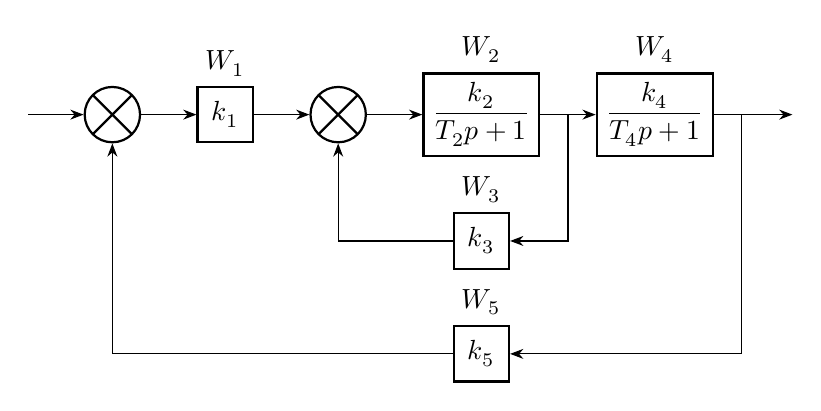
\begin{tikzpicture}[
        > = Stealth,
        input/.style = {
          coordinate
        },
        output/.style = {
          coordinate
        },
        block/.style = {
          draw,
          thick,
          rectangle,
          minimum height = 2em,
          minimum width = 2em,
        },
        sum/.style = {
          draw,
          thick,
          circle,
          path picture = {
            \draw[black]
            (path picture bounding box.south east)
            -- (path picture bounding box.north west)
            (path picture bounding box.south west)
            -- (path picture bounding box.north east);
          },
          minimum height = 2em,
        },
      ]
        % First layer
        \node [input, anchor = north west] (input) {};
        \node [sum, right = 2em of input.east, anchor = west]
          (s1) {};
        \node [block, right = 2em of s1.east, anchor = west, label = $W_1$]
          (w1) {$k_1$};
        \node [sum, anchor = west, right = 2em of w1.east]
          (s2) {};
        \node [block, anchor = west, right = 2em of s2.east, label = $W_2$] (w2)
          {$\displaystyle\frac{k_2}{T_2 p + 1}$};
        \node [block, anchor = west, right = 2em of w2.east, label = $W_4$] (w4)
          {$\displaystyle\frac{k_4}{T_4 p + 1}$};

        \node[output, right = of w4] (out) {};

        % layer 2
        \node [block, below = 2em of w2.south, label = $W_3$]
          (w3) {$k_3$};

        % layer 3
        \node [block, below = 2em of w3, label = $W_5$]
          (w5) {$k_5$};

        % Edges
        \draw [->] (input) -- (s1);
        \draw [->] (s1) -- (w1);
        \draw [->] (w1) -- (s2);
        \draw [->] (s2) -- (w2);
        \draw [->] (w2) -- (w4);
        \draw [->] (w4) -- node[name=phantom] {} (out);

        \draw [->] (w2.east) ++(1em, 0) |- (w3);
        \draw [->] (w3.west) -| (s2.south);

        \draw [->] (w4.east) ++(1em, 0) |- (w5);
        \draw [->] (w5.west) -| (s1.south);
      \end{tikzpicture}
      \caption{Задана структурна схема системи управління}
      \label{fig:task}
    \end{figure}

    \noindent{}Спростимо контур~$W_2 W_3$ в~еквівалентну ланку~$W_{23}$:
    \begin{IEEEeqnarray*}{rCl}
      W_{23} &=&
              \frac{W_2}{1 - W_2 W_3}
              =
              \frac{
                \frac{k_2}{T_2 p + 1}
              }{
                1 - k_3 \cdot \frac{k_2}{T_2 p + 1}
              }
              =
              \frac{
                k_2
              }{
                T_2 p + 1
              }
              \cdot
              \frac{
                1
              }{
                1 - \frac{k_2 k_3}{T_2 p + 1}
              }
              \\
             &=&
              \frac{
                k_2
              }{
                T_2 p + 1
              }
              \cdot
              \frac{
                1
              }{
                \frac{
                  T_2 p + 1
                }{
                  T_2 p + 1
                }
                -
                \frac{k_2 k_3}{T_2 p + 1}
              }
              =
              \frac{
                k_2
              }{
                T_2 p + 1
              }
              \cdot
              \frac{
                1
              }{
                \frac{
                  T_2 p + 1
                  -
                  k_2 k_3
                }{
                  T_2 p + 1
                }
              }
              \\
            &=&
              \frac{
                k_2
              }{
                T_2 p + 1
              }
              \cdot
              \frac{
                T_2 p + 1
              }{
                (T_2 p + 1)
                -
                k_2 k_3
              }
             =
              \frac{
                k_2
              }{
                T_2 p + 1
                -
                k_2 k_3
              }
             .
    \end{IEEEeqnarray*}

    \noindent{}Тоді отримаємо спрощену еквівалентну схему~(рис.~\ref{fig:s01}).
    \begin{figure}[!htbp]
      \centering
      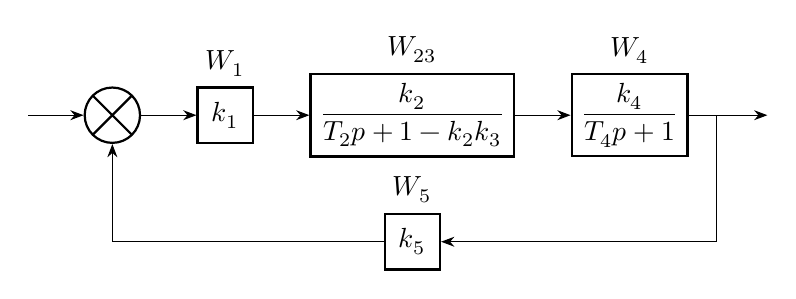
\begin{tikzpicture}[
        > = Stealth,
        input/.style = {
          coordinate
        },
        output/.style = {
          coordinate
        },
        block/.style = {
          draw,
          thick,
          rectangle,
          minimum height = 2em,
          minimum width = 2em,
        },
        sum/.style = {
          draw,
          thick,
          circle,
          path picture = {
            \draw[black]
            (path picture bounding box.south east)
            -- (path picture bounding box.north west)
            (path picture bounding box.south west)
            -- (path picture bounding box.north east);
          },
          minimum height = 2em,
        },
      ]
        % First layer
        \node [input, anchor = north west] (input) {};
        \node [sum, right = 2em of input.east, anchor = west]
          (s1) {};
        \node [block, right = 2em of s1.east, anchor = west, label = $W_1$]
          (w1) {$k_1$};
        \node [block, anchor = west, right = 2em of w1.east, label = $W_{23}$]
          (w23) {$\displaystyle\frac{ k_2 }{ T_2 p + 1 - k_2 k_3 }$};
        \node [block, anchor = west, right = 2em of w23.east, label = $W_4$] (w4)
          {$\displaystyle\frac{k_4}{T_4 p + 1}$};

        \node[output, right = of w4] (out) {};

        % layer 3
        \node [block, below = 2em of w23.south, label = $W_5$]
          (w5) {$k_5$};

        % Edges
        \draw [->] (input) -- (s1);
        \draw [->] (s1) -- (w1);
        \draw [->] (w1) -- (w23);
        \draw [->] (w23) -- (w4);
        \draw [->] (w4) -- node[name=phantom] {} (out);

        \draw [->] (w4.east) ++(1em, 0) |- (w5);
        \draw [->] (w5.west) -| (s1.south);
      \end{tikzpicture}
      \caption{Структурна схема системи управління після спрощення контуру~$W_2 W_3$ в~еквівалентну ланку~$W_{23}$}
      \label{fig:s01}
    \end{figure}

    \noindent{}Спростимо послідовність ланок~$W_1 W_{23} W_4$ в~еквівалентну ланку~$W_{1234}$:
    \begin{IEEEeqnarray*}{rCl}
      W_{1234} &=& W_1 W_{23} W_4
                =
                k_1
                \cdot
                \frac{
                  k_2
                }{
                  T_2 p + 1
                  -
                  k_2 k_3
                }
                \cdot
                k_4
                =
                \frac{
                  k_1
                  k_2
                  k_4
                }{
                  T_2 p + 1
                  -
                  k_2 k_3
                }
               .
    \end{IEEEeqnarray*}

    \noindent{}Спростивши послідовність ланок~$W_1 W_{23} W_4$ в~еквівалентну ланок~$W_{1234}$, отримаємо спрощену еквівалентну схему~(рис.~\ref{fig:s02}).
    \begin{figure}[!htbp]
      \centering
      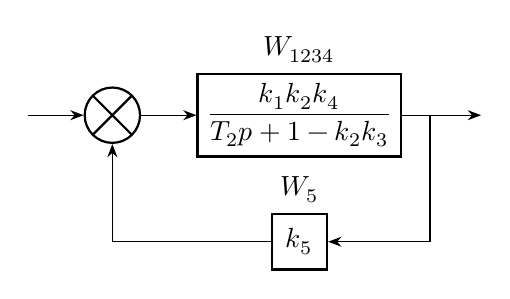
\begin{tikzpicture}[
        > = Stealth,
        input/.style = {
          coordinate
        },
        output/.style = {
          coordinate
        },
        block/.style = {
          draw,
          thick,
          rectangle,
          minimum height = 2em,
          minimum width = 2em,
        },
        sum/.style = {
          draw,
          thick,
          circle,
          path picture = {
            \draw[black]
            (path picture bounding box.south east)
            -- (path picture bounding box.north west)
            (path picture bounding box.south west)
            -- (path picture bounding box.north east);
          },
          minimum height = 2em,
        },
      ]

        % First layer
        \node [input, anchor = north west] (input) {};
        \node [sum, right = 2em of input.east, anchor = west]
          (s1) {};
        \node [block, right = 2em of s1.east, anchor = west, label = $W_{1234}$]
          (w1234) {$\displaystyle\frac{ k_1 k_2 k_4 }{ T_2 p + 1 - k_2 k_3 }$};

        \node[output, right = of w1234] (out) {};

        % layer 3
        \node [block, below = 2em of w1234.south, label = $W_5$]
          (w5) {$k_5$};

        % Edges
        \draw [->] (input) -- (s1);
        \draw [->] (s1) -- (w1234);
        \draw [->] (w1234) -- (out);

        \draw [->] (w1234.east) ++(1em, 0) |- (w5);
        \draw [->] (w5.west) -| (s1.south);
      \end{tikzpicture}
      \caption{Структурна схема системи управління після спрощення контуру~$W_1 W_{23} W_4$ в~еквівалентну ланку~$W_{1234}$}
      \label{fig:s02}
    \end{figure}

    \noindent{}Спростимо контур~$W_{1234} W_5$ в~еквівалентну ланку~$W_{12345}$:
    \begin{IEEEeqnarray*}{rCl}
      W_{12345} &=& \frac{
                    W_{1234}
                  }{
                    1 - W_{1234} W_5
                  }
                 =
                 \frac{
                   k_1
                   k_2
                   k_4
                 }{
                   T_2 p + 1
                   -
                   k_2 k_3
                 }
                 \cdot
                 \frac{
                   1
                 }{
                   1
                   -
                   \frac{
                     k_1
                     k_2
                     k_4
                   }{
                     T_2 p + 1
                     -
                     k_2 k_3
                   }
                 }
                 \\
                &=&
                 \frac{
                   k_1
                   k_2
                   k_4
                 }{
                   T_2 p + 1
                   -
                   k_2 k_3
                 }
                 \cdot
                 \frac{
                   1
                 }{
                   \frac{
                     T_2 p + 1
                     -
                     k_2 k_3
                   }{
                     T_2 p + 1
                     -
                     k_2 k_3
                   }
                   -
                   \frac{
                     k_1
                     k_2
                     k_4
                   }{
                     T_2 p + 1
                     -
                     k_2 k_3
                   }
                 }
                 \\
                &=&
                 \frac{
                   k_1
                   k_2
                   k_4
                 }{
                   T_2 p + 1
                   -
                   k_2 k_3
                 }
                 \cdot
                 \frac{
                   1
                 }{
                   \frac{
                     T_2 p + 1
                     -
                     k_2 k_3
                     -
                     k_1
                     k_2
                     k_4
                   }{
                     T_2 p + 1
                     -
                     k_2 k_3
                   }
                 }
                 \\
                &=&
                 \frac{
                   k_1
                   k_2
                   k_4
                 }{
                   (T_2 p + 1)
                   -
                   k_2 k_3
                 }
                 \cdot
                 \frac{
                   T_2 p + 1
                   -
                   k_2 k_3
                 }{
                   T_2 p + 1
                   -
                   k_2 k_3
                   -
                   k_1
                   k_2
                   k_4
                 }\\
                &=&
                 \frac{
                   k_1
                   k_2
                   k_4
                 }{
                   T_2 p + 1
                   -
                   k_2 k_3
                   -
                   k_1
                   k_2
                   k_4
                 }
               .
    \end{IEEEeqnarray*}

    \noindent{}Тоді отримаємо спрощену еквівалентну схему~(рис.~\ref{fig:s03}).
    \begin{figure}[!htbp]
      \centering
      \begin{tikzpicture}[
        > = Stealth,
        input/.style = {
          coordinate
        },
        output/.style = {
          coordinate
        },
        block/.style = {
          draw,
          thick,
          rectangle,
          minimum height = 2em,
          minimum width = 2em,
        },
        sum/.style = {
          draw,
          thick,
          circle,
          path picture = {
            \draw[black]
            (path picture bounding box.south east)
            -- (path picture bounding box.north west)
            (path picture bounding box.south west)
            -- (path picture bounding box.north east);
          },
          minimum height = 2em,
        },
      ]

        % First layer
        \node [input, anchor = north west] (input) {};
        \node [block, right = 2em of input, anchor = west, label = $W_{12345}$]
          (w12345) {$\displaystyle\frac{ k_1 k_2 k_4 }{ T_2 p + 1 - k_2 k_3 - k_1 k_2 k_4 }$};

        \node[output, right = of w12345] (out) {};

        % Edges
        \draw [->] (input) -- (w12345);
        \draw [->] (w1234) -- (out);
      \end{tikzpicture}
      \caption{Структурна схема системи управління після спрощення контуру~$W_{1234}W_5$ в~еквівалентну ланку~$W_{12345}$}
      \label{fig:s03}
    \end{figure}

    \noindent{}Отже, так~ми~визначили, що~передаточна функція заданої системи управління виглядає так: $W(p) = \left. k_1 k_2 k_4 \middle/ {T_2 p + 1 - k_2 k_3 - k_1 k_2 k_4} \right. $.

\end{document}
